%=========================================================================
% (c) 2011, 2012 Josef Lusticky <xlusti00@stud.fit.vutbr.cz>

\chapter{NTP client in Contiki OS}
%!Distinguish between TIME and CLOCK

For implementation of a reasonably useful NTP client
operating system must meet conditions listed in appendix~\ref{app:requirements}.
The main problem for NTP client implementation in Contiki is a total
lack of time support.
Not only no common interface availability but also
almost no platform-specific code has been implemented towards time support yet.
Contiki provides basic clock interface particularly for use of timers though.
This interface is common for all supported platforms,
but the particular implementation is platform specific.

Another deal is possible packet loss if communication uses UDP on transport layer.
The reason this can happen often is explained in section~\ref{sec:contiki-uip}.

For developing and testing Contiki NTP client the AVR Raven platform with ATmega1284P~\cite{avr-datasheet} was used.
% do not mention, appendix?
How to get a working setup with Contiki on this platform is described in
%!%% CHECK THIS %%%
docs/setup.pdf file on the CD enclosed to this thesis.
%%% CHECK THIS %%%

\section{Required hardware clock interface}
Contiki features a basic clock interface with a simple goal - measuring time.
This interface provides needed calls for timers and its definition is to be found in {\it{/core/sys/clock.h}} file.
Specific implementations of this common interface are located in {\it{/cpu}} directory of Contiki source code.
The interface provides call for initialising CPU's clock system - {\it{clock\_init}}, that is automatically called during
boot sequence of Contiki.
The goal of the {\it{clock\_init}} call is to set up
appropriate timer/counter registers and interrupt service routines.
On AVR CPU this call is implemented as C macro which evaluates to specific setup code for each CPU
when compiling.
The setup code is not common to all CPUs because of differences among them - e.g. there are usually
only three Timer/Counter modules, but AVR ATmega1284P has four Timer/Counter modules~\cite{avr-datasheet}.

%At least one of those is always 16 bit wide
%This extra module on AVR ATmega1284P is used for
% three vs. 3

%clock\_seconds
%CLOCK\_SECOND
This is however enough for implementing a reasonable time interface and using it for NTP client later.

% ntp interface extending the clock library, similar to posix calls

%!!AVR

Adjusting time - COMPARE\_REGISTER = 31 => 128Hz => 1s = 1s
COMPARE\_REGISTER = 31 => ca132.129Hz => 1s = ca1.032s
COMPARE\_REGISTER = 33 => 124.12per => 1s = 0.96p


\section{Operating system clock interface}
There is no way of setting the time in Contiki OS.
The interface for setting, getting and adjusting time was developed in this thesis.

The structure similar to POSIX {\it{timespec}} structure (described in section~\ref{sec:posix})
was implemented for expressing exact time value.
However name was changed to {\it{time\_spec}} to avoid collision with existing POSIX-compliant systems.
\begin{lstlisting}
struct time_spec {
  unsigned long sec;
  unsigned long nsec;
};
\end{lstlisting}
The structure representing time specification uses unsigned long values.
The value 0 seconds and 0 nanoseconds is equal to Unix prime epoch (1st January 1970).
In case of seconds part, the 32-bit unsigned long value was chosen because the existing value
{\it{seconds}}, representing uptime in Contiki, is of the same type.
Such time representation will wrap around in year 2106.
In case of nanoseconds part, the 32-bit unsigned long value was chosen because there is no need
for negative values.
As the 32-bit unsigned long type can express values from 0 to $2^{32}$-1 (4~294~967~295),
and one second has 1~000~000~000 nanoseconds, this will never wrap around.
Even negative results of subtraction work after casting the result to singed type
because 1~000~000~000 is still less than maximum expressible value of signed long type $2^{31}$-1 (2~147~483~647).
The nanosecond precision was chosen as modern systems also aim towards this precision~\cite{posix,ntp-precision} and
the microsecond precision would also require at least 32-bit data type -
one second has 1~000~000 microseconds, which is more than maximum expressible value of signed 16-bit
type $2^{16}$ (65~536).

It should be noted that unsigned long data type does not have to always result in 32-bit variable -
it is up to compiler what data width it chooses for each data type.
But as ISO C99 standard states, the maximum value for an object of type unsigned long
shall be greater or equal $2^{32}$-1 (4~294~967~295)~\cite{c99}.
This in fact results in at least 32-bit variable unless the compilation setting is changed.
Next to this, as the already presented variable {\it{seconds}} is also of unsigned long type,
the value {\it{sec}} in {\it{time\_spec}} structure and {\it{boottime}}
shall be of the same type as arithmetic operations are made on them.

\begin{lstlisting}
void
clock_set_time(unsigned long sec)
{
  boottime = sec - seconds;
}
\end{lstlisting}

\begin{lstlisting}
void
clock_get_time(struct time_spec *ts)
{
  ts->sec = boottime + seconds;
  ts->nsec = (unsigned long) ((1000000000 / CLOCK_SECOND) * scount);
}
\end{lstlisting}
%The interface for getting the time simply adds value when system was booted...
E.g. assuming the code is compiled using GCC version 4.3.5,
multiplication of two unsigned long variable takes 33 instructions including {\it{call}} and {\it{ret}}
instructions for entering and returning from the {\it{\_\_mulsi3}} routine, which computes
the result of multiplication.
%avr-objdump
According to AVR Instruction Set manual~\cite{avr-instruction-set} this results in 48 clock cycles overhead,
which takes 3~000 nanoseconds assuming 16MHz CPU clock.
The timestamp provided is therefore not exact.
However there is no correction to remove this inaccuracy,
instead the application must be aware that the timestamp is not exactly accurate.


\section{NTP values}
Unlike the RFC 5905~\cite{rfc5905} shows, there are no 64 bit values. %! RFC - A.4. Kernel System Clock Interface
No floating point numbers.
Divide by 2 is done through arithmetic right shift. Compiler does not translates division by 2 automatically.

\section{NTP client implementation}
Structures representing NTP message were borrowed from OpenNTPD NTP Unix daemon.
%They are not using the GCC extension for representing a bit field.

Packet sanity tests~\cite{ntp-arch}.

A client sends messages to each server with a poll interval of $2^{\tau}$
seconds, as determined by the poll exponent $\tau$ (tau).
In NTPv4, $\tau$ ranges from 4 (16 s) to 17 (36 h).


% filling the packet
Precision express strictly speaking elapsed time to read the system clock from userland~\cite{ntp-arch}.
However most implementation supply clock precision.
%Dragonfly BSD:
%wmsg.precision = -6;
%Chrony, NTP.org - getting resolution, gettimeofday, clock_getres
\begin{lstlisting}
// set clock precision - convert Hz to log2 - borrowed from OpenNTPD
int b = CLOCK_SECOND; // CLOCK_SECOND * OCR2A
int a;
for (a = 0; b > 1; a--, b >>= 1)
  {}
msg.precision = a;
\end{lstlisting}
This will work for clock precision greater or equal 1s, i.e. CLOCK\_SECOND must be greater or equal 1.
%refer to CLOCK\_SECOND - is always greater or equal 1

The clock are set if the time difference is greater than XX seconds. %! TODO
\begin{lstlisting}
if (labs((signed long) (ts.sec - tmpts.sec)) > 2)
{
  clock_set_time(ts.sec);
}
\end{lstlisting}
Even if {\it{tmpts.sec}} value is greater than {\it{ts.sec}} value,
subtracting and casting to signed type gives correct (negative) result~\cite{c99}.
Assuming 32-bit data types this will work until 2038 when wrap around can occur due to difference
between {\it{ts.sec}} and {\it{tmpts.sec}} greater than $2^{31}$-1 (2~147~483~647).
But as NTP Era 0 ends 2036 the NTP client code must be changed in the future anyway.

%! TODO

\section{Communication}
% IEEE 802.15.4
%as RFC~4944 written by 6lowpan working group of IETF
%made the underlaying IEEE 802.15.4 layer
%look like an IPv6 link~\cite{6lowpan} and
\begin{figure}
  \centering
  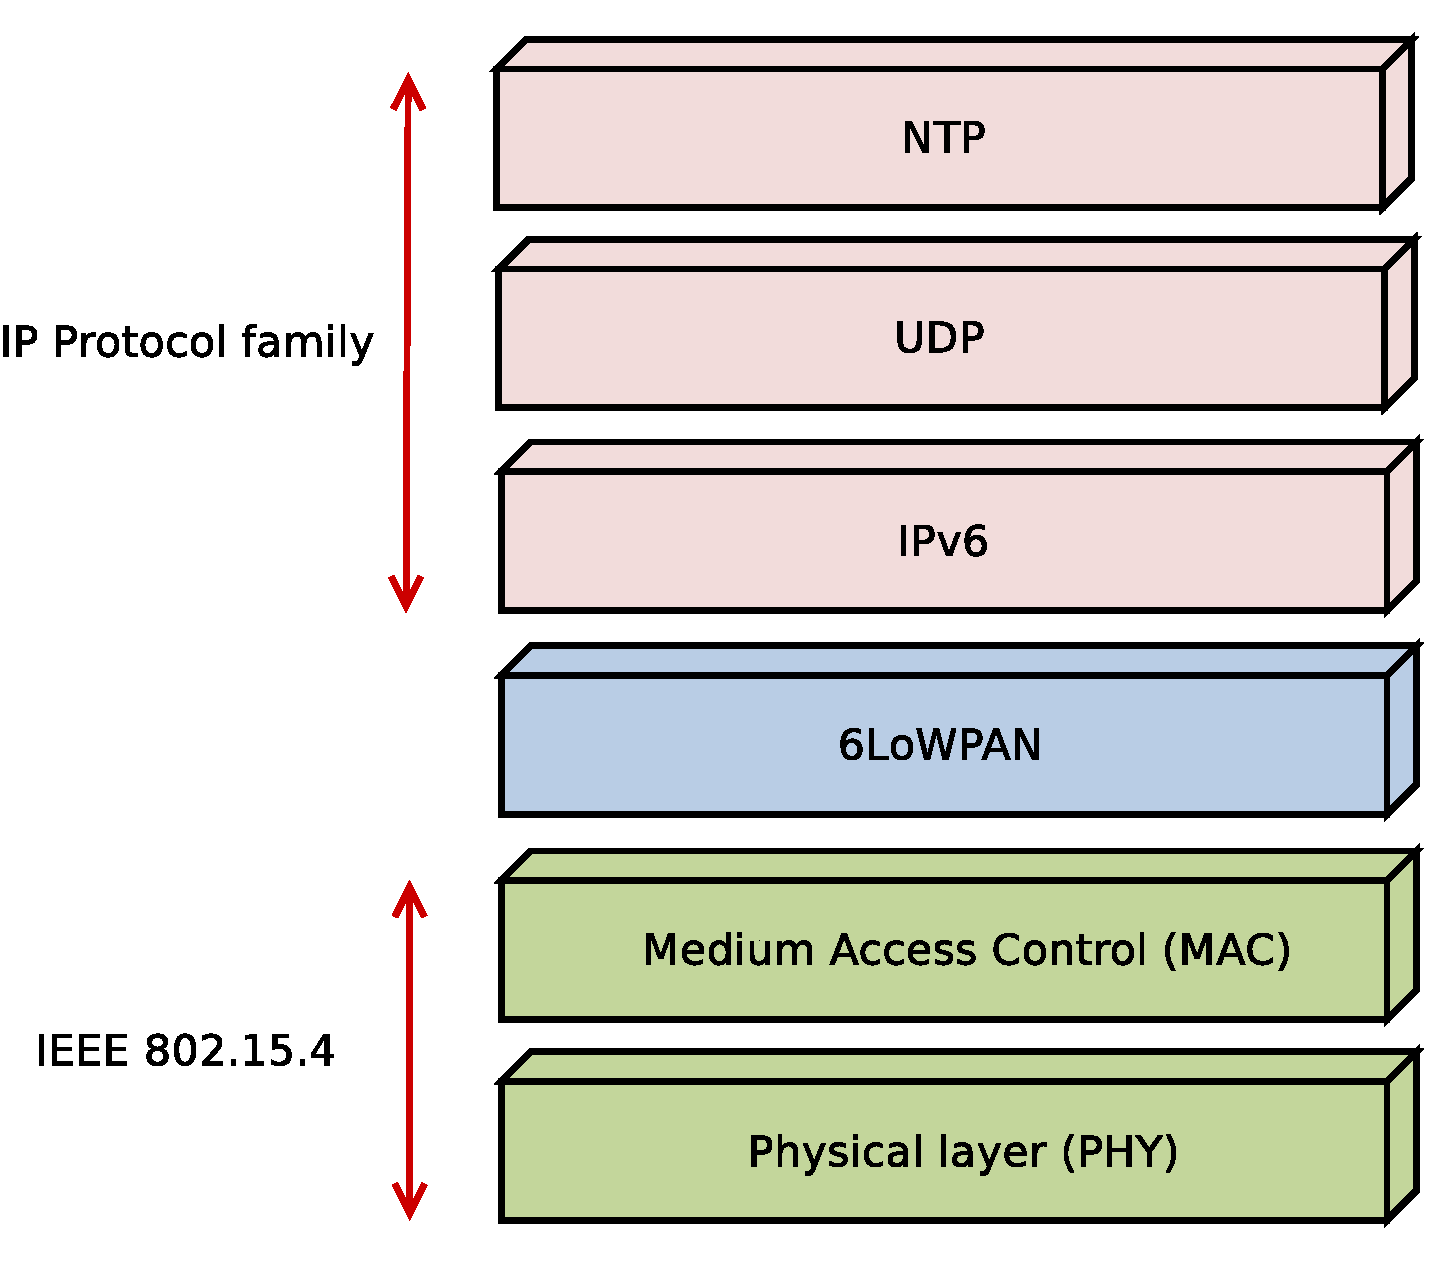
\includegraphics[width=9cm,keepaspectratio]{fig/6lowpan.pdf}
  \caption{Communication stack with 6lowpan layer}
  \label{fig:implementation-6lowpan}
  \bigskip
\end{figure}

% There is no IPv4 support...


\section{Network communication over UDP transport layer}
The uIP packet buffer is accessed through
the uip\_buf array and is used to hold incoming and outgoing packets.
The device driver should place incoming data into this buffer.
When sending data, the device driver should read the link
level headers and the TCP/IP headers from this buffer.
The size of the link level headers is configured by the UIP\_LLH\_LEN
define and in case of ethernet it is 14.

The application data need not be placed in this buffer, so
the device driver must read it from the place pointed to by the
uip\_appdata pointer %as illustrated by the following example:
